\documentclass[12pt, a4paper]{article}
\usepackage{a4wide}

\usepackage[utf8]{inputenc}
\usepackage[ngerman]{babel}
\usepackage[T1]{fontenc}
\usepackage{palatino} %font

\usepackage{graphicx}
\usepackage{caption}
\usepackage{subcaption} %für subfigures
\usepackage{url}
\usepackage{tocloft}
\usepackage{acronym}
\usepackage{float}
\usepackage{color} 

\usepackage[babel,german=quotes,threshold=3]{csquotes} 

\usepackage{lipsum}
\usepackage{hyperref}  %hyperref still needs to be put at the end!

%Pfad für Grafiken
\graphicspath{{img/}}

%Styleregeln
\widowpenalty10000 % Vermeidet einzelne Zeilen eines Absatzes zu Beginn einer Seite
\clubpenalty10000 % Vermeidet einzelne Zeilen eines Absatzes am Ende einer Seite
\addtocontents{toc}{\protect\sloppy}
\setcounter{tocdepth}{3}

\begin{document}

%deaktiviere Seitenzahlen
\pagenumbering{gobble}

%Titelseite
\begin{titlepage}
\centering
\thispagestyle{empty}
\begin{center}

\includegraphics[width=0.9\textwidth]{uos.pdf}
\end{center}
\LARGE{\textsc{Institut für Informatik\\Arbeitsgruppe Verteilte Systeme}}
\vfill
\LARGE{\emph{Seminar}}\\
\LARGE{\emph{Mobility and Traffic in Computer Networks}}\\
\vspace{8mm}
\huge{\textbf{{\fontfamily{ppl}\selectfont
Analyzing Mobility-Traffic Correlations in Large WLAN Traces}}}\\
\vspace{9mm}
\LARGE{Tim Bohne}\\
\vspace{0.2cm}
%ACHTUNG: !!!Matrikelnummer nur für die Abgabeversion, NICHT mit ins Wiki hochladen!!!
% \normalsize{Matrikelnummer}\\
\vspace{4cm}
\large{Sommersemester 2019}\\
\vspace{0.2cm}
\large{\today}
\vfill
\end{titlepage}
\newpage

%Inhaltsverzeichnis
\tableofcontents
\newpage

\pagestyle{plain}
\pagenumbering{arabic} %Starte Seitennummerierung

\section{Einleitung}

Die stetig wachsende Zahl mobiler Geräte führt zu enormen Herausforderungen bei der Entwicklung
und Planung der dafür erforderlichen Infrastruktur. Beim Konzipieren neuer Netzwerke ist es von zentraler
Bedeutung, diese in möglichst realistischer Weise zu simulieren, um sinnvolle Designentscheidungen
treffen zu können. Dabei spielen zwei Bereiche eine essenzielle Rolle, die Bewegung der Nutzer bzw. Geräte
sowie der Datenverkehr innerhalb des Netzwerks.\newline
Diese Ausarbeitung befasst sich mit Korrelationen zwischen diesen beiden Bereichen,
welche primär anhand der Ergebnisse des Papers \textquote{Flutes vs. Cellos: Analyzing Mobility-Traffic
Correlations in Large WLAN Traces} \cite{Alipour2018} aus dem Jahr 2018 erörtert werden.
Ziel des Papers ist im Wesentlichen, einen ersten Schritt in Richtung integrierter Mobilitäts-Datenverkehr-Modelle 
zu ermöglichen, um in der Zukunft realistischere Test-Szenarien und Benchmarks zu entwickeln.
Darüber hinaus werden an einigen Stellen weiterführende Quellen einbezogen.
\newline\newline
Zunächst werden in Kapitel \ref{sec:basics} die Grundlagen der Mobilität und des Datenverkehrs in Rechnernetzen
eingeführt. Anschließend geht es in Kapitel \ref{sec:correlations} um Korrelationen zwischen beiden
Bereichen, die anhand der Ergebnisse von \cite{Alipour2018} erörtert werden.
Darauffolgend werden einige Aspekte diskutiert, bevor schließlich in \ref{sec:conclusion} ein abschließendes
Fazit und ein Ausblick formuliert wird.

\section{Grundlagen}
\label{sec:basics}

Bevor Korrelationen zwischen Datenverkehr und Mobilität im WLAN sinnvoll thematisiert werden können, 
werden in diesem Kapitel zunächst die Grundlagen beider Konzepte eingeführt.
In Abschnitt \ref{sec:mobility} geht es um Mobilität in Drahtlosnetzwerken und Abschnitt \ref{sec:traffic} handelt
vom Datenverkehr in ebensolchen.

\subsection{Mobilität}
\label{sec:mobility}

Die Performanz eines kabellosen Kommunikationsnetzwerks hängt unter anderem von der Bewegung 
der Nutzer bzw. Geräte innerhalb dieses Netzwerks ab. Dementsprechend ist es erstrebenswert,
z.B. bei der Planung neuer Netze Simulationen mit möglichst realistischen Bewegungsmustern durchzuführen.
Ein Mobilitätsmodell beschreibt das Bewegungsmuster mobiler Benutzer bzw. Geräte,
also die Art, in welcher sich deren Standort, Geschwindigkeit und Beschleunigung im Laufe der Zeit ändern. \cite{Camp2002}
In \cite{Camp2002} wird dabei zwischen zwei grundsätzlichen Modellen unterschieden, den \textquote{Entity-Mobility-Models},
also Modellen, bei denen die Bewegung einzelner Entitäten modelliert wird und den \textquote{Group-Mobility-Models},
bei welchen es darum geht, die Bewegung einer Gruppe von Nutzern bzw. Geräten zu modellieren,
in welcher die Bewegung der einzelnen Entitäten voneinander abhängt.\newline
Neben der Unterscheidung zwischen Entity- und Group-Mobility-Modellen, wird dort außerdem zwischen zwei Arten der Datenbasis unterschieden,
welche der Simulation zugrunde liegt. Es gibt zum einen die Bewegungsmodelle, die auf Trace-Daten basieren, d.h. auf Beobachtungen
der Bewegung von Nutzern in tatsächlich existierenden Systemen. Diese liefern bei einer ausreichend großen Gruppe von Nutzern
und einer ausreichend langen Beobachtungsphase sehr akurate Informationen, setzen allerdings voraus, dass ein solches Netzwerk
bereits existiert. \cite{Camp2002} Zum anderen existieren Modelle mit synthetischen Bewegungsmustern für Netzwerkumgebungen, 
für die noch keine Traces vorliegen. Dabei geht es darum, die Bewegung der Nutzer möglichst realistisch abzubilden,
wofür es verschiedene Arten von Ansätzen gibt.\newline
Wie in \cite{Aschenbruck2011} geschildert, können synthetische Modelle bestimmte Abhängigkeiten modellieren.
Zeitliche Abhängigkeiten sorgen z.B. dafür, dass die Bewegung einer Entität durch dessen Bewegung in der Vergangenheit
beeinflusst wird. Außerdem können räumliche Abhängigkeiten darfür sorgen, dass die Bewegung einer Entität durch die umgebenden 
Entitäten beeinflusst wird (Group-Mobility). Auch geographische Restriktionen können Teil des Modells sein.
Des Weiteren wird in \cite{Aschenbruck2011} darauf hingewiesen, dass auch Modelle wie
\textquote{Random-Waypoint} und \textquote{Random-Walk} existieren, welche keine dieser Abhängigkeiten
aufweisen. Diese Modelle sind einfach zu implementieren, jedoch nicht sehr realistisch.
Insgesamt existiert eine Vielzahl von Mobilitätsmodellen mit verschiedenen Ansätzen,
auf welche zum Teil im Verlauf dieser Ausarbeitung an geeigneter Stelle eingegangen wird.

\subsection{Datenverkehr}
\label{sec:traffic}

Zu einer sinnvollen Evaluation der Performanz eines Kommunikationssystems gehört auch die Simulation des Datenverkehrs
innerhalb dieses Systems. Wie bereits bei der Bewegungsmodellierung, kann auch hier von tatsächlichen Beobachtungen in
existierenden Netzen ausgegangen werden, sofern diese vorliegen.
\newline\newline
Einfacher Datenverkehr besteht aus einzelnen Ankünften diskreter Entitäten.
Bei diesen Entitäten kann es sich z.B. um Pakete handeln. Darüber hinaus gibt es Datenverkehr, 
bei welchem mehrere Entitäten zusammen in sogenannten \textquote{Batch-Arrivals} eintreffen.
Im einfachsten Fall wird in einer Simulation eine zufällige Sequenz von Zwischenankunftszeiten \footnote{Zeit zwischen zwei 
aufeinanderfolgenden \textquote{Arrivals}.} generiert. Neben Ankunftszeiten und Batch-Größen ist es zudem häufig sinnvoll,
die Last zu modellieren. \cite{Frost1994} Die Last wird in \cite{Frost1994} als die Menge der Arbeit $W_n$ im System beschrieben,
die die $n$-te eintreffende Entität erfordert.
\newline\newline
Ein einfaches Modell des Datenverkehrs ist \textsc{CBR} (Constant Bitrate), bei welchem eine Anzahl von Paketankünften
pro Zeiteinheit definiert wird. Die Paketgröße ist dabei ebenfalls konstant. Dieses Modell ist sehr simpel und dementsprechend
leicht zu implementieren, dafür jedoch in der Regel nicht besonders realistisch.\newline
Neben \textsc{CBR}- gibt es den typischerweise realistischeren \textsc{VBR}-Traffic (Variable Bitrate), 
welcher z.B. beim Videostreaming auftritt, bei dem kodierte Frames eine variable, zufällige Größe besitzen.\cite{Frost1994}
Um einen realistischen, heterogenen Traffic-Mix zu erhalten, sollten in einem Modell laut \cite{Frost1994} verschiedene
Ströme des Datenverkehrs gemultiplext werden, z.B. Sprachverbindungen, Video-Übertragungen und Datei-Transporte.
\newline\newline
Eine weitere wichtige Eigenschaft des Datenverkehrs ist die sogenannte \textquote{Burstiness}, also die Stoßhaftigkeit.
Traffic entsteht in Schüben, z.B. für komprimierte Videos und Datentransfers. Die Ankünfte der Pakete bilden visuelle
Cluster. Der Datenverkehr in Breitbandnetzen wird von dieser Art Traffic dominiert. \cite{Frost1994}
\newline\newline
Wie bereits bei der Bewegungsmodellierung gibt es auch hier eine Vielzahl verschiedener Modelle, die in bestimmten Szenarien
geeignet sein können, um realistischen Datenverkehr zu modellieren.

\section{Korrelationen zwischen Mobilität und Datenverkehr}
\label{sec:correlations}

Wie in den Abschnitten \ref{sec:mobility} und \ref{sec:traffic} eingeführt, hängt die Performanz eines mobilen
Netzwerks erheblich von den Mustern der Mobilität und des Datenverkehrs innerhalb des Netzwerks ab.
\cite{Alipour2018} untersuchen mögliche Korrelationen zwischen beiden Faktoren.
\newline\newline
Aktuelle Modelle betrachten entweder die Mobilität oder den Datenverkehr, erfassen jedoch nicht das Zusammenspiel beider Faktoren.
Außerdem verwenden viele trace-basierte Mobilitätsmodelle Datensätze aus der Prä-Smartphone-Ära,
was die heutige Relevanz dieser Modelle in Frage stellt. \cite{Alipour2018}\newline
Die Autoren von \cite{Alipour2018} beschäftigen sich mit Mobilitäts- und Datenverkehrmodellen für Laptops und Smartphones.
Die Modelle sind datengetrieben, es werden $30$\textsc{TB} große Datensätze von $300$\textsc{K} Geräten betrachtet, 
welche auf einem Campusgelände betrieben wurden. Zur Analyse dieser Daten wurde das Framework FLAMeS (\textbf{F}ramework for 
\textbf{L}arge-scale \textbf{A}nalysis of \textbf{M}obil\textbf{e} \textbf{S}ocieties) entwickelt.
Im Folgenden werden relevante Aspekte und Ergebnisse aus der Veröffentlichung zusammengefasst.\newline\newline
Dass die beiden Faktoren der Mobilität und des Datenverkehrs sich trotz der bisher überwiegend isolierten Betrachtungen
durchaus gegenseitig beeinflussen, veranschaulichen die Autoren durch folgende alltägliche Beispiele. 
Eine Person verlangsamt ihren Gang, wenn diese eine Nachricht erhält. Ebenso kann die Netzwerkaktivität von der
Mobilität und Position abhängen. Stationäre Nutzer konsumieren und produzieren in der Regel mehr Daten als jene, 
die sich bewegen. Außerdem verwenden Personen an unterschiedlichen Orten unterschiedliche Anwendungen.
Diese simplen Beispiele lassen eine gemeinsame Betrachtung beider Faktoren bereits als sinnvoll erscheinen.
Um diesen Zusammenhang genauer zu untersuchen, unterscheiden sie zwischen stationären Geräten (Laptops) und mobilen Geräten
(Smartphones). Da Laptops auch durchaus als mobil angesehen werden können, präzisieren die Autoren die Unterscheidung
durch \textquote{on-the-go}- und \textquote{stop-to-use}-Geräte. Das Framework FLAMeS ermöglicht es, stationäre und
mobile Geräte zu differenzieren und in Bezug auf ihren Datenverkehr und ihre Mobilität zu untersuchen.
Im Kern untersuchen die Autoren dabei drei Fragestellungen:

\begin{itemize}
    \item Wie unterscheiden sich Mobilitäts- und Datenverkehr-Charakteristiken zwischen unterschiedlichen Geräteklassen,
    Zeiten und Orten?
    \item Wie stehen diese Charakteristiken zueinander in Beziehung?
    \item Sollten neue Modelle entwickelt werden, die diese Unterschiede berücksichtigen?
\end{itemize}

Das FLAMeS-Systems besteht aus drei Phasen, in der ersten Phase findet die Datensammlung und ein Preprocessing statt.
Anschließend kommt es in der zweiten Phase zur Mobilitäts- und Traffic-Analyse, wobei zwischen Laptops und Smartphones
unterschieden wird. In der letzten Phase findet schließlich eine integrierte Analyse der Mobilität und des Traffics statt.
% \begin{figure}[H]
% \centering
% 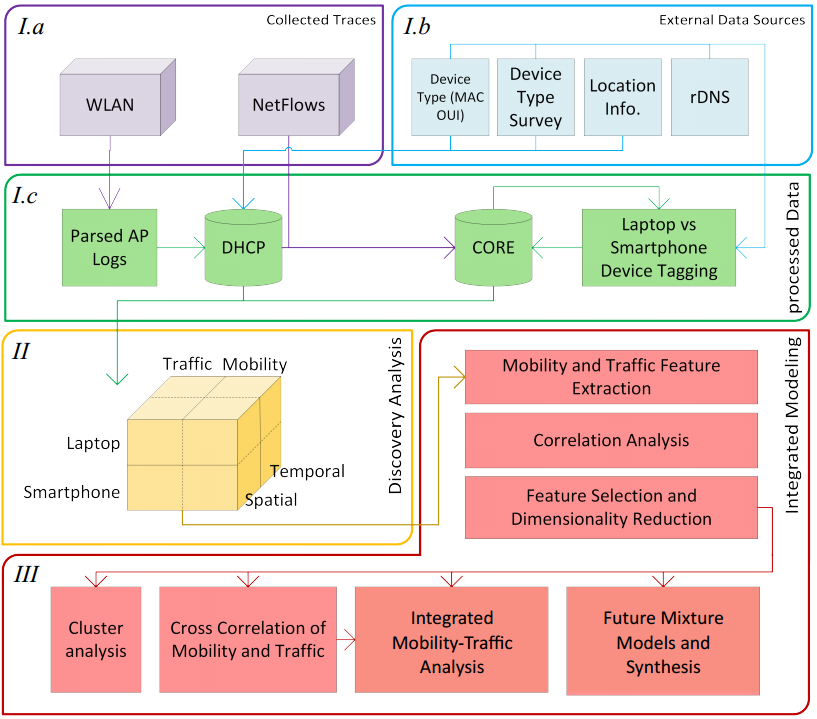
\includegraphics[width=0.65\textwidth]{img/FLAMeS.png}
% \caption{FLAMeS-System. \cite{Alipour2018}}
% \label{fig:flames}
% \end{figure}

\subsection{Datensammlung und Preprocessing}

Die gesammelten Daten stammen aus zwei Quellen. Die erste Quelle sind WLAN-AP\footnote{Access-Point}-Logs. 
Diese Logs wurden an $1760$ APs in $138$ Gebäuden über $479$ Tage auf dem
Campus einer Universität aufgezeichnet. Die Daten stammen von insgesamt $316$\textsc{K} Geräten aus den Jahren $2011$ und $2012$.
Jeder Eintrag enthält die MAC-Adresse des Geräts, dessen zugewiesene IP-Adresse, den AP, mit welchem das Gerät verbunden ist
und einen Zeitstempel.
Die Orte der APs werden durch die Längen- und Breitengrade der Gebäude, in welchen sie sich befinden, mithilfe der Google Maps API
approximiert. Daneben gibt es als weitere Quelle Netflow-Logs. Im selben Netzwerk wurden im April $2012$ über $76$ Mrd.
Einträge in Netflow-Traces gesammelt. Ein \textquote{Flow} entspricht einer konsekutiven Sequenz von Paketen mit demselben
Transportprotokoll, Start- und Ziel-IP und Port. \cite{Alipour2018}
Anschließend werden die Netflow-Einträge durch das dynamische MAC-to-IP Mapping aus den DHCP-Logs mit den WLAN-Verbindungen aus den AP-Logs gematcht. Die Ergebnisse werden mittels rDNS\footnote{Reverse DNS} durch Ort und Webseiten-Informationen ergänzt. \cite{Alipour2018}
Darauffolgend geht es darum, die Geräte in Laptops und Smartphones zu klassifizieren.
Zunächst kann der Hersteller des Geräts mit der OUI \footnote{Organizationally Unique Identifier - 24-Bit-Zahl, 
die eindeutig den Hersteller identifiziert.} basierend auf den ersten drei Oktetten der MAC-Adresse identifiziert werden.
Da viele Hersteller nur einen Gerätetyp herstellen, können auf diese Weise bereits
$46 \%$ der Geräte klassifiziert werden. Die Heuristik, welche von den Autoren zur Klassifizierung verwendet wird,
prüft zusätzlich, ob ein Gerät \textit{admob.com} kontatktiert, eine sehr verbreitete Plattform für Werbung auf Mobilgeräten.
Ist dies der Fall, so wird ein Gerät als Mobilgerät klassifiziert. Auf diese Weise konnten $86 \%$ der Geräte in den AP-Logs
und $97 \%$ der Netflow-Traces klassifiziert werden. Diese Art der Geräteklassifizierung wahre im Gegensatz zur Analyse von 
HTTP-Headern, die möglicherweise zu noch genaueren Ergebnissen führt, die Privatsphäre der Nutzer.\newline
Wie man Abb. \ref{fig:traces} entnehmen kann, ist die Anzahl der Flows und der
Gesamt-Traffic bei Laptops deutlich höher als bei Mobilgeräten, obwohl es insgesamt deutlich mehr verbundene Mobilgeräte gibt.
Wie zu erwarten treten die Peaks an Wochentagen auf. Dass die Netzwerkaktivität nach dem 25. abnimmt, liegt daran, dass dort
die vorlesungsfreie Zeit beginnt.

\begin{figure}[H]
    \centering
    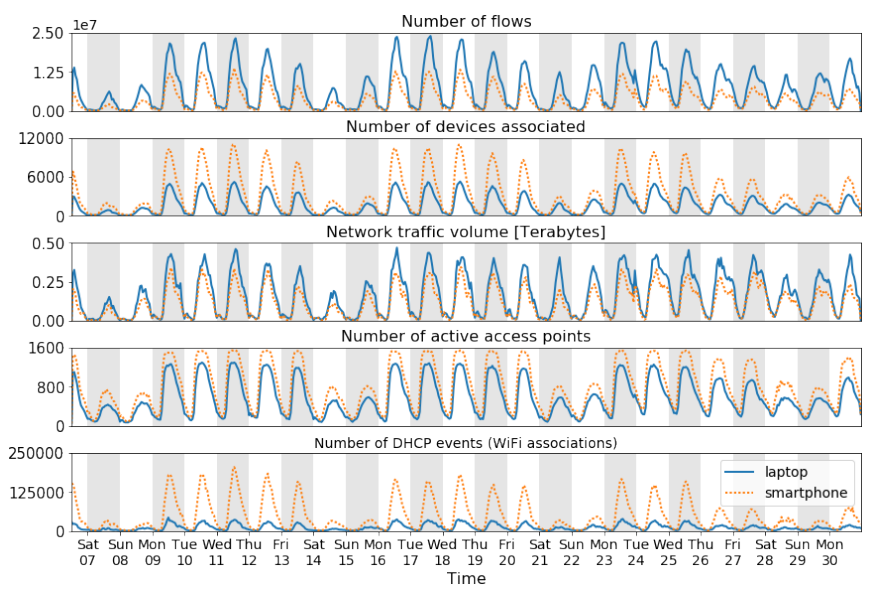
\includegraphics[width=0.65\textwidth]{img/traces.png}
    \caption{Kombinierte WLAN-AP- und Netflow-Traces über $25$ Tage. \cite{Alipour2018}}
    \label{fig:traces}
\end{figure}

\subsection{Mobilitätsanalyse}

In diesem Abschnitt werden die Ergebnisse der Mobilitätsanalyse aus \cite{Alipour2018} zusammengefasst, in denen es
um die zeitliche und räumliche Analyse der Mobilität der verschiedenen Geräteklassen geht.
Die Startzeiten von WLAN-Sessions stimmen in Gebäuden, in denen Vorlesungen stattfinden mit den Startzeiten der Vorlesungen überein.
In diesen Gebäuden fällt die Aktivität von Laptops nach dem Ende der Vorlesungszeiten stark, während die Aktivität von Mobilgeräten
noch etwas länger erhalten bleibt. Für die Bibliothek und soziale Einrichtungen auf dem Campus ist die Wahrscheinlichkeit
für neue Sessions später am Abend höher. Diese Ergebnisse treffen nur auf Wochentage zu, deren Ablauf durch
die Vorlesungszeiten eine gewisse Struktur erhält.
Dies hat außerdem zur Folge, dass Stundenten, die an Vorlesungen teilnehmen, an Wochentagen einen eingeschränkteren Bewegungsradius haben.
Die Autoren haben die räumliche Ausbreitung der Geräte über einen Zeitraum von $6$ Monaten analysiert.
Nach einer initialen Phase von ca. einer Woche stabilisiert sich diese Ausbreitung. Für Laptops findet eine 
substanzielle Reduktion der Gesamtmobilität statt, während diese bei Smartphones nicht in einer solchen Deutlichkeit vorliegt.
Da Smartphones \textquote{always-on}-Geräte sind, ist es leichter, deren Mobilität zu erfassen, da sie auch an Orten
wie Bushaltestellen etc., an denen Laptops typischerweise nicht eingeschaltet sind, verbunden sind.
Dies ermöglicht eine genauere Erfassung der Mobilität dieser Geräte.
Außerdem wird die Anzahl der unterschiedlichen besuchten Gebäude eines Nutzers gezählt und ein bevorzugtes
Gebäude dieses Nutzers als jenes definiert, in welchem dieser an einem Tag die meiste Zeit verbracht hat.
Dazu werden die Session-Zeiten innerhalb eines Gebäudes aufsummiert.
Laptops haben etwas längere Aufenthaltszeiten und werden in der Regel verwendet, wenn Nutzer länger an einem Ort verweilen.

\subsection{Trafficanalyse}

In diesem Abschnitt geht es um die zeitliche und räumliche Analyse des Datenverkehrs der verschiedenen Geräteklassen.
Im Folgenden werden die Ergebnisse der Traffic-Analyse von \cite{Alipour2018} vorgestellt.
Eine relevante Charakteristik ist die \textquote{Flow-Size}, also die Summe der Bytes aller Pakete eines Flows.
An Wochentagen ist die durchschnittliche Größe von Flows bei Smartphones mehr als doppelt so groß wie jene von Laptop-Flows.
Auch an Wochenenden ändert sich dies nicht signifikant. Die durchschnittliche Paketgröße von Smartphone-Flows
ist ca. $50 \%$ größer als die von Laptops. Die Median-Größe der Pakete von Smartphones fällt an Wochenenden, 
während diese bei Laptops gleich bleibt. Laptop-Flows zeigen zwischen Wochentagen und Wochenden in Bezug auf
die durchschnittliche Paketgröße keine signifikante Veränderung.
Trotz kleinerer Flows generiert ein durchschnittlicher Laptop $2.7$ mal so viel Traffic wie ein durchschnittliches Smartphone,
weil ein Laptop für $3.7$ mal so viele Flows verantwortlich ist, wie ein Smartphone.
\newline\newline
Ebenfalls interessant ist die Laufzeit eines Flows. Beide Gerätetypen zeigen erhöhte Mittelwerte an Wochenenden.
Da es zusätzlich weniger aktive Geräte an Wochenenden gibt, ist für die verbleibenden aktiven Geräte eine erhöhte Aktivität
zu beobachten. Smartphones zeigen insgesamt mehr extreme Phasen der Inaktivität, die unter anderem durch größere
Mobilität und Paketverluste verursacht werden können.
Auch die verwendeten Protokolle sind von Interesse. TCP ist für $78.5 \%$ der Laptop-Flows verantwortlich
und für $98.2 \%$ der Smartphone-Flows. Die höhere Präsenz von UDP bei Laptops ist zu erwarten, weil
UDP-Verbindungen, die z.B. bei Multiplayer-Spielen, Video-Konferenzen und Filesharing auftreten,
typischerweise weniger auf Mobilgeräten stattfinden.
Außerdem wurde die Last an den APs in sämtlichen Gebäuden täglich beobachtet. Dabei wurde darauf geachtet,
die Beobachtungen außerhalb der Klausurenphase zu tätigen, um Veränderungen im Verhalten der Nutzer zu vermeiden.
Es wurde die tägliche Rate der Paket- und Flowankünfte an den APs betrachtet. Die Median Flowraten sind
$42$\textsc{K} bzw. $20$\textsc{K} für Laptops und Smartphones an Wochentagen ($7.5$\textsc{K} bzw. $0.5$\textsc{K}
an Wochenenden). Die durchschnittliche Anzahl von Laptop-Paketen, die täglich von APs verarbeitet werden,
ist $1.6$ mal größer als die von Smartphones. An Wochenenden wird ein großer Anteil der APs nicht verwendet,
was die Aussage einer geringeren Mobilität der Nutzer an Wochenenden unterstützt.
Das tatsächliche Traffic-Volumen der APs beträgt an durchschnittlichen Wochentagen für $90 \%$ der APs
weniger als $5$\textsc{GB} Laptop-Traffic ($2.5$\textsc{GB} an Wochenenden) und weniger als $3$\textsc{GB} Smartphone-Traffic
($1$\textsc{GB} an Wochenenden).
Auch das Verhalten der Nutzer ist relevant. An Wochentagen \textcolor{red}{konsumieren} $90 \%$ der Laptops weniger als $700$\textsc{MB},
während $90 \%$ der Smartphones weniger als $200$\textsc{MB} verbrauchen.
Ein ähnliches Bild ergibt sich bei der Paketrate. An Wochentagen generieren Laptops durchschnittlich $318$\textsc{K} Pakete, 
während Smartphones nur durchschnittlich $84$\textsc{K} Pakete am Tag generieren. 
An Wochenenden erhöht sich die Paketrate und der Datenkonsum der wenigen verbleibenden Laptops deutlich,
während bei den Smartphones nur leichte Veränderungen zu beobachten sind.
Weiterhin gut geeignet, um Unterschiede zwischen Laptops und Smartphones zu verdeutlichen, sind die tatsächlichen Aktivitätszeiten.
Dabei werden die Netflows herangezogen und nicht die WLAN-AP-Verbindungszeiten, denn dies ermöglicht es \textquote{Idle}-Zeiten
von aktiven Zeiten zu unterscheiden. Laptops haben verglichen mit Smartphones $4x$ höhere durchschnittliche Aktivitätszeiten.
Insgesamt sind über $90 \%$ der Laptops weniger als $3.5$ Stunden am Tag aktiv und $90 \%$ der Smartphones weniger als eine Stunde.\newline
Zusammenfassend lässt sich sagen, dass der Datanverbrauch von Smartphones mehr bursty mit größeren Flows und kleinerer aktiver
Dauer ist. Außerdem sind an Wochenenden weniger Geräte am Campus, aber jene die verbleiben, sind überdurchschnittlich aktiv 
und konsumieren überdurchschnittlich viele Daten. Insgesamt ist festzuhalten, dass Smartphones mobiler sind, 
eine größere Anzahl von APs besuchen, größere Flow-Sizes haben und trotzdem für insgesamt weniger Netzwerklast 
verantwortlich sind.

\subsection{Integrierte Mobilitäts- und Traffic-Modelle}

Zuletzt wird in \cite{Alipour2018} untersucht, ob es einen Bedarf für integrierte Mobility-Traffic-Modelle gibt.
Um die Analyse und Interpretation zu vereinfachen und die wichtigsten Eigenschaften zu identifizieren,
wird mithilfe des \textsc{CFS}\footnote{Correlation Feature Selection}-Algorithmus \textquote{Feature-Engineering} betrieben. 
\newline\newline
\textbf{Mobilität}\newline
Der \textsc{CFS}-Algorithmus wird mit $8$ Eigenschaften ausgeführt
und liefert $5$ verbleibende Eigenschaften, die für eine kombinierte Analyse geeignet sind.
An Wochentagen gibt es eine starke Korrelation zwischen der Zeit, die im bevorzugten Gebäude 
verbracht wird und der Dauer der Session, jedoch nur eine schwache Korrelation an Wochenenden, was darauf hindeutet,
dass die meiste Onlinezeit am Wochenende im bevorzugten Gebäude verbracht wird.
\newline\newline
\textbf{Traffic}\newline
Beim Traffic wird der \textsc{CFS}-Algorithmus mit $19$ Eigenschaften ausgeführt, die auf $11$
reduziert werden. Auch beim Traffic existieren Korrelationen, die wohl interessanteste Erkenntnis ist allerdings, dass die
Aktivitätszeiten und die Anzahl von Flows und Paketen nur schwach korreliert, was bedeutet, dass Nutzer,
die länger online sind, nicht notwendigerweise mehr Traffic erzeugen.
\newline\newline
Ein wichtiger Schritt in Richtung integrierter Mobility-Traffic-Models ist die Analyse der Korrelationen
zwischen beiden Dimensionen (Mobilität und Traffic) basierend auf der Teilmenge der Eigenschaften,
die vom \textsc{CFS}-Algorithmus ausgewählt wurden.\newline
Die Ergebnisse lassen sich wie folgt zusammenfassen. Smartphones haben hohe Scores bei den Mobilitätsmetriken, besitzen eine
insgesamt kleinere Anzahl von Flows und weniger Netzwerktraffic, aber produzieren im Durchschnitt größere Flows.
Für Laptops gilt an Wochenenden, je mehr Zeit in bevorzugten Gebäuden verbracht wird, desto größer die Gesamtaktivitätszeit
und Flow-Anzahl. Dieser Effekt existiert in abgeschwächter Form auch bei Smartphones. 
An Wochentagen existieren diese Korrelationen nicht.\newline
Mittels Machine Learning wurde untersucht, wie sich Mobilitäts- und Traffic-Features zwischen
Smartphones und Laptops unterscheiden. Anschließend wurde nach natürlichen konvexen Clustern von Usern im
Datensatz gesucht. Diese Schritte verifizieren, dass die Unterschiede der Mobilitäts- und Traffic-Charakteristiken
zwischen den Gerätetypen signifikant sind.

\textbf{Supervised Classification}\newline
Die Autoren haben Support Vector Maschinen (SVM) auf verschiedenen Teilmengen von Features
verwendet, um die Zulässigkeit der Gerätetyp-Inferenz und die Beziehung zwischen Mobilitäts- und Traffic-Charakteristiken
zu untersuchen. Insgesamt wurde die Genauigkeit verschiedener Modelle analysiert. Dabei hat sich herausgestellt,
dass kombinierte Modelle, die sowohl Traffic, als auch Mobilität berücksichtigen genauer sind,
als isolierte Modelle. Außerdem erhöht sich die Genauigkeit weiter, wenn zwischen Wochentagen und Wochenenden differenziert wird.
Das deutet daraufhin, dass das Nutzerverhalten für beide Gerätetypen besser unterscheidbar ist, wenn kombinierte
Traffic und Mobilitäts-Features betrachtet werden, besonders, wenn Wochentage isoliert von Wochenenden betrachtet werden.
\newline\newline
\textbf{Unsupervised Clustering}\newline
Um natürliche konvexe Cluster zu untersuchen, wurde der K-means-Algorithmus verwendet.
Wenn nur Mobilitäts-Features verwendet werden, werden ca. $60 \%$ der Geräte korrekt geclustert.
Werden dagegen nur Traffic-Features genutzt, erreicht man eine Genauigkeit von $81.2 \%$.
Werden Mobilität und Traffic kombiniert, erhöht sich die Genauigkeit auf $81.5 \%$.
\newline\newline
\textbf{Mixture Model}\newline
Um einen Schritt in Richtung der Synthetisierung von Traces basierend auf den Datasets zu machen,
wurden Gaussian Mixture Models (GMM) mit kombinierten Mobilitäts- und Traffic-Features trainiert.
Anschlißend wurde Kolmogorov-Smirnov (KS) Statistik verwendet, um die generierten Samples zu Echtdaten zu vergleichen.
Dabei hat sich herausgestellt, dass das kombinierte Modell in der Lage ist, das Verhalten beider Gerätetypen zu abzubilden.
Das kombinierte Modell produziert Samples, dessen Traffic-Features den Originaldaten besser entsprechen, als ein GMM,
welches nur mit Traffic-Features trainiert wurde, was darauf hindeutet, dass eine Beziehung zwischen Mobilität und Traffic besteht.
Allerdings bringt das GMM des kombinierten Modells verglichen mit dem Modell, welches ausschließlich Mobility-Features trainiert wurde,
keine Verbesserung.
\newline\newline
Insgesamt besteht ein signifikantes Potenzial integrierter Mobilitäts- und Traffic-Modelle, welche die Unterschiede
und Beziehungen von Features zwischen Gerätetypen, Zeit und Ort besser abbilden können als isolierte Modelle.

\subsection{Diskussion}

In \cite{Alipour2018} wurde die Frage gestellt, ob es sinnvoll ist, Modelle zu entwickeln, die sowohl
Mobilitäts-, als auch Datenverkehrcharakteristiken berücksichtigen. Es wurde darin gezeigt, dass solche
kombinierten Betrachtungen potenziell zu deutlich realistischeren Ergebnissen gelangen können,
als die in der Regel zu simplen isolierten Betrachtungen.\newline
Es wurde ein Framework entwickelt, um die Datensätze eines bestehenden Netzwerks dahingehend zu analysieren.
Zunächst ging es dabei um Geräteklassifizierung und anschließend um eine Untersuchung der Mobilitäts-
und Traffic-Metriken, wobei die verschiedenen Gerätetypen über Raum und Zeit hinweg miteinander verglichen wurden.
Nachdem gezeigt wurde, dass es signifikante Unterschiede zwischen den Gerätetypen gibt,
wurde mittels Machine-Learning ein gemischtes Modell trainiert, welches Datenpunkte generiert
und es konnte gezeigt werden, dass kombinierte Mobilitäts- und Traffic-Features die Unterschiede in den
Metriken besser abbilden, als isolierte Modelle. Die eingangs erwähnten Fragestellungen wurden beantwortet
und es wurden erste Schritte in Richtung integrierter Mobilitäts- und Traffic-Modelle getan.

\section{Fazit und Ausblick}
\label{sec:conclusion}

Bereits das alltägliche Beispiel der Person, die ihren Gang verlangsamt um eine empfangene Nachricht zu lesen,
verdeutlicht, dass es einen Zusammengang zwischen Mobilität und Datenverkehr bei Mobilgeräten gibt.
In \cite{Alipour2018} wird diese intuitive Idee eines Zusammenhangs bestätigt. Da beide Bereiche
bisher typischerweise isoliert voneinander betrachtet werden, handelt es sich um ein aktives Forschungsfeld,
bei dem in Zukunft weitere Betrachtungen und konkretere Ansätze kombinierter Modelle zu erwarten sind.

Die Autoren der in Abschnitt \ref{sec:} vorgestellten Veröffentlichung haben eine erweiterte Version veröffentlicht,
in welcher sie tiefer auf bestimmte zuvor betrachtete Aspekte eingehen...

\vfill
\pagebreak

%Bibliographie
\addcontentsline{toc}{section}{Literatur}
\bibliographystyle{IEEEtranSA}
%\bibliographystyle{acm}
\bibliography{sources.bib}

\end{document}
